\documentclass{article}
\usepackage{enumerate}
\usepackage{graphicx}
\usepackage{float}

\usepackage{amsmath}
\usepackage[margin=1in]{geometry}
\usepackage[parfill]{parskip}

\title{Physics 112 Problem Set 9 \\ \large{Holzapfel, Section 102}}
\author{Sahil Chinoy}
\date{November 13, 2017}

\begin{document}
\maketitle{}

\begin{enumerate}

	\item

	The chemical potential of both the Fermi and Bose gases in the classical regime ($n \ll n_Q$) is given by $\mu = \tau \log (n_Q/n) \propto \log(1/N)$ for fixed $T, V$.

	The chemical potential of a Bose gas in the quantum regime ($n \gg n_Q$) is given by $\mu = \epsilon_0 - (\tau/N)$, so it asymptotically approaches the ground state energy $\epsilon_0$ as $N \to \infty$.

	\begin{figure}[H]
	\caption{$\mu$ versus $N$ for a Bose gas}
	\centering
	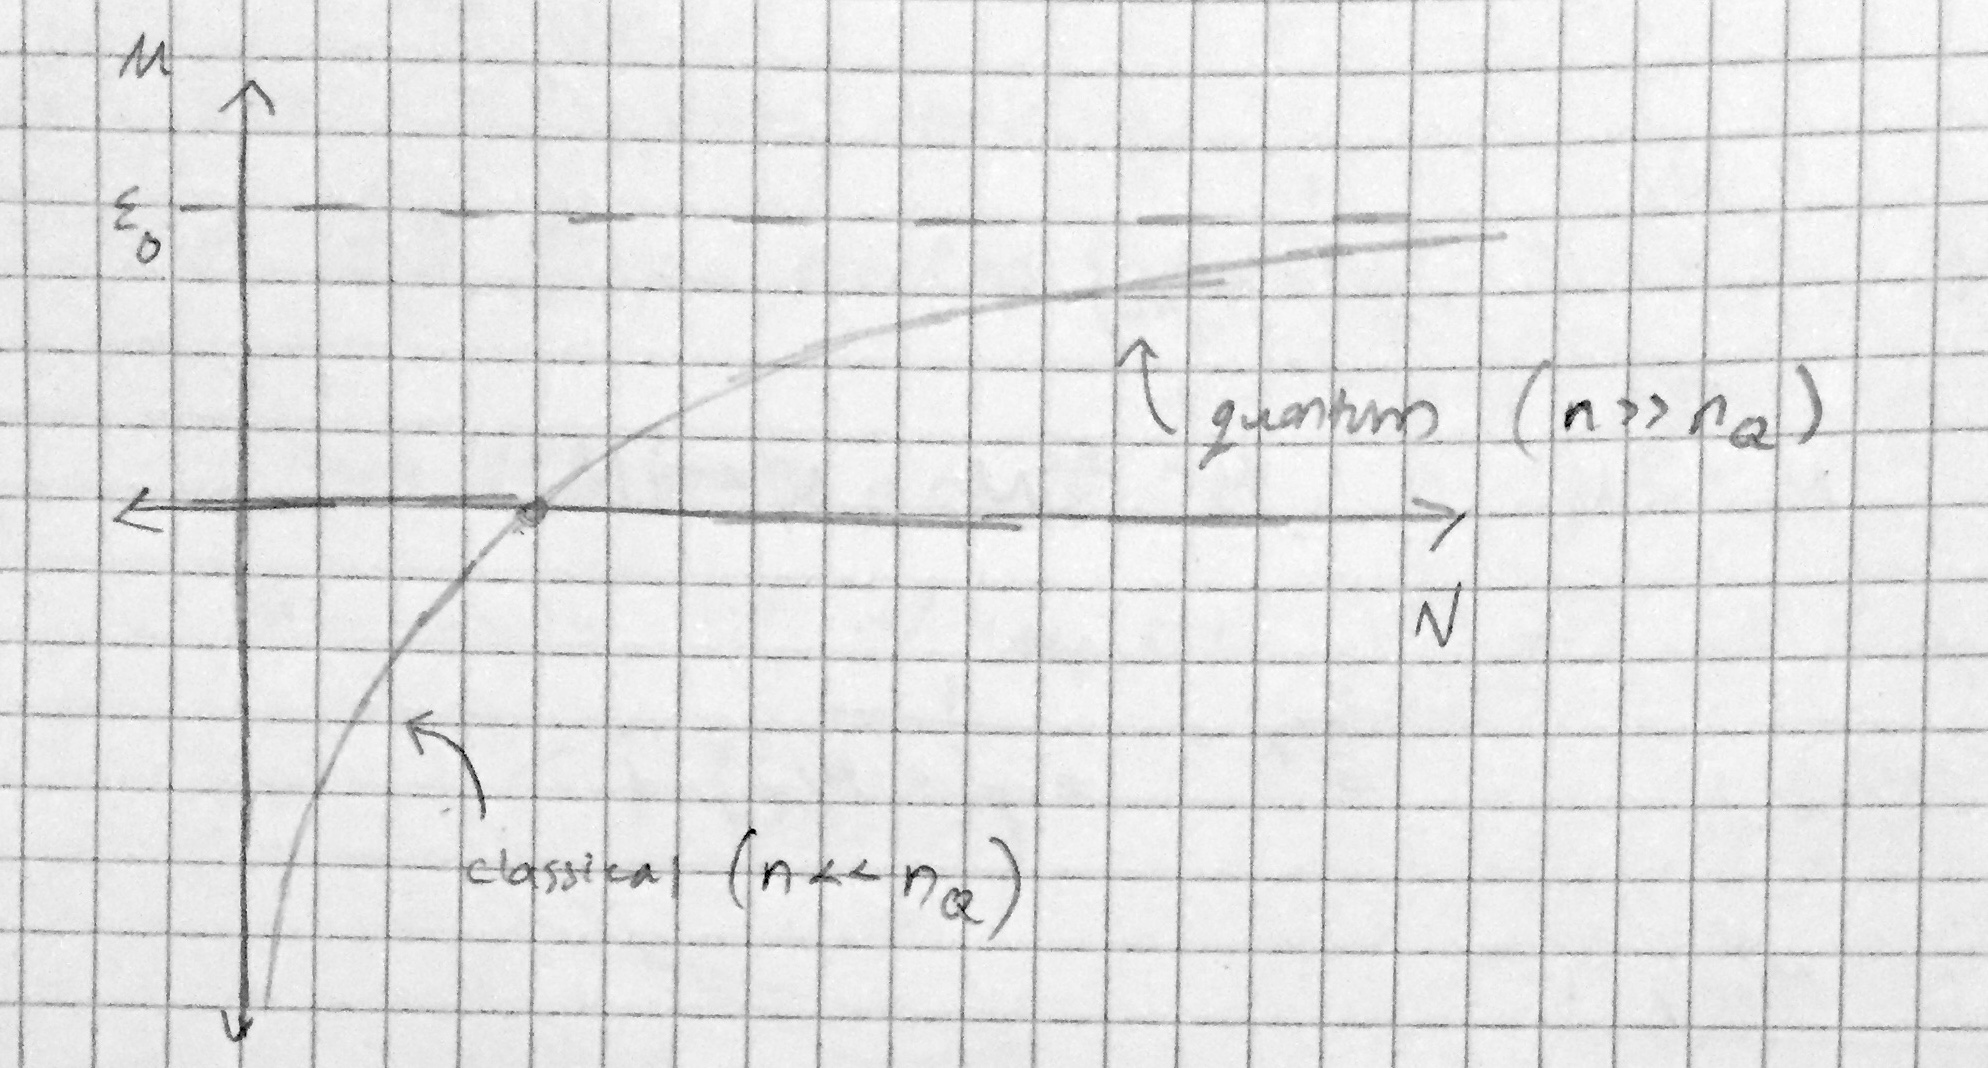
\includegraphics[width=12cm]{img/bose}
	\end{figure}

	For the Fermi gas, we can find the chemical potential with the integral

	$$N = \int \limits_0^\infty d\epsilon \mathcal{D}(\epsilon) f(\epsilon, \tau, \mu) \propto \int \limits_0^\infty d\epsilon \frac{\epsilon^{1/2}}{\exp((\epsilon-\mu)/\tau)} = \int \limits_0^\mu \epsilon^{1/2} d\epsilon \propto \mu^{3/2},$$

	to leading order (by way of a Sommerfeld expansion). So the chemical potential of a Fermi gas in the quantum regime is given by $\mu \propto N^{2/3},$ so it increases without bound as $N \to \infty$. 

	\begin{figure}[H]
	\caption{$\mu$ versus $N$ for a Fermi gas}
	\centering
	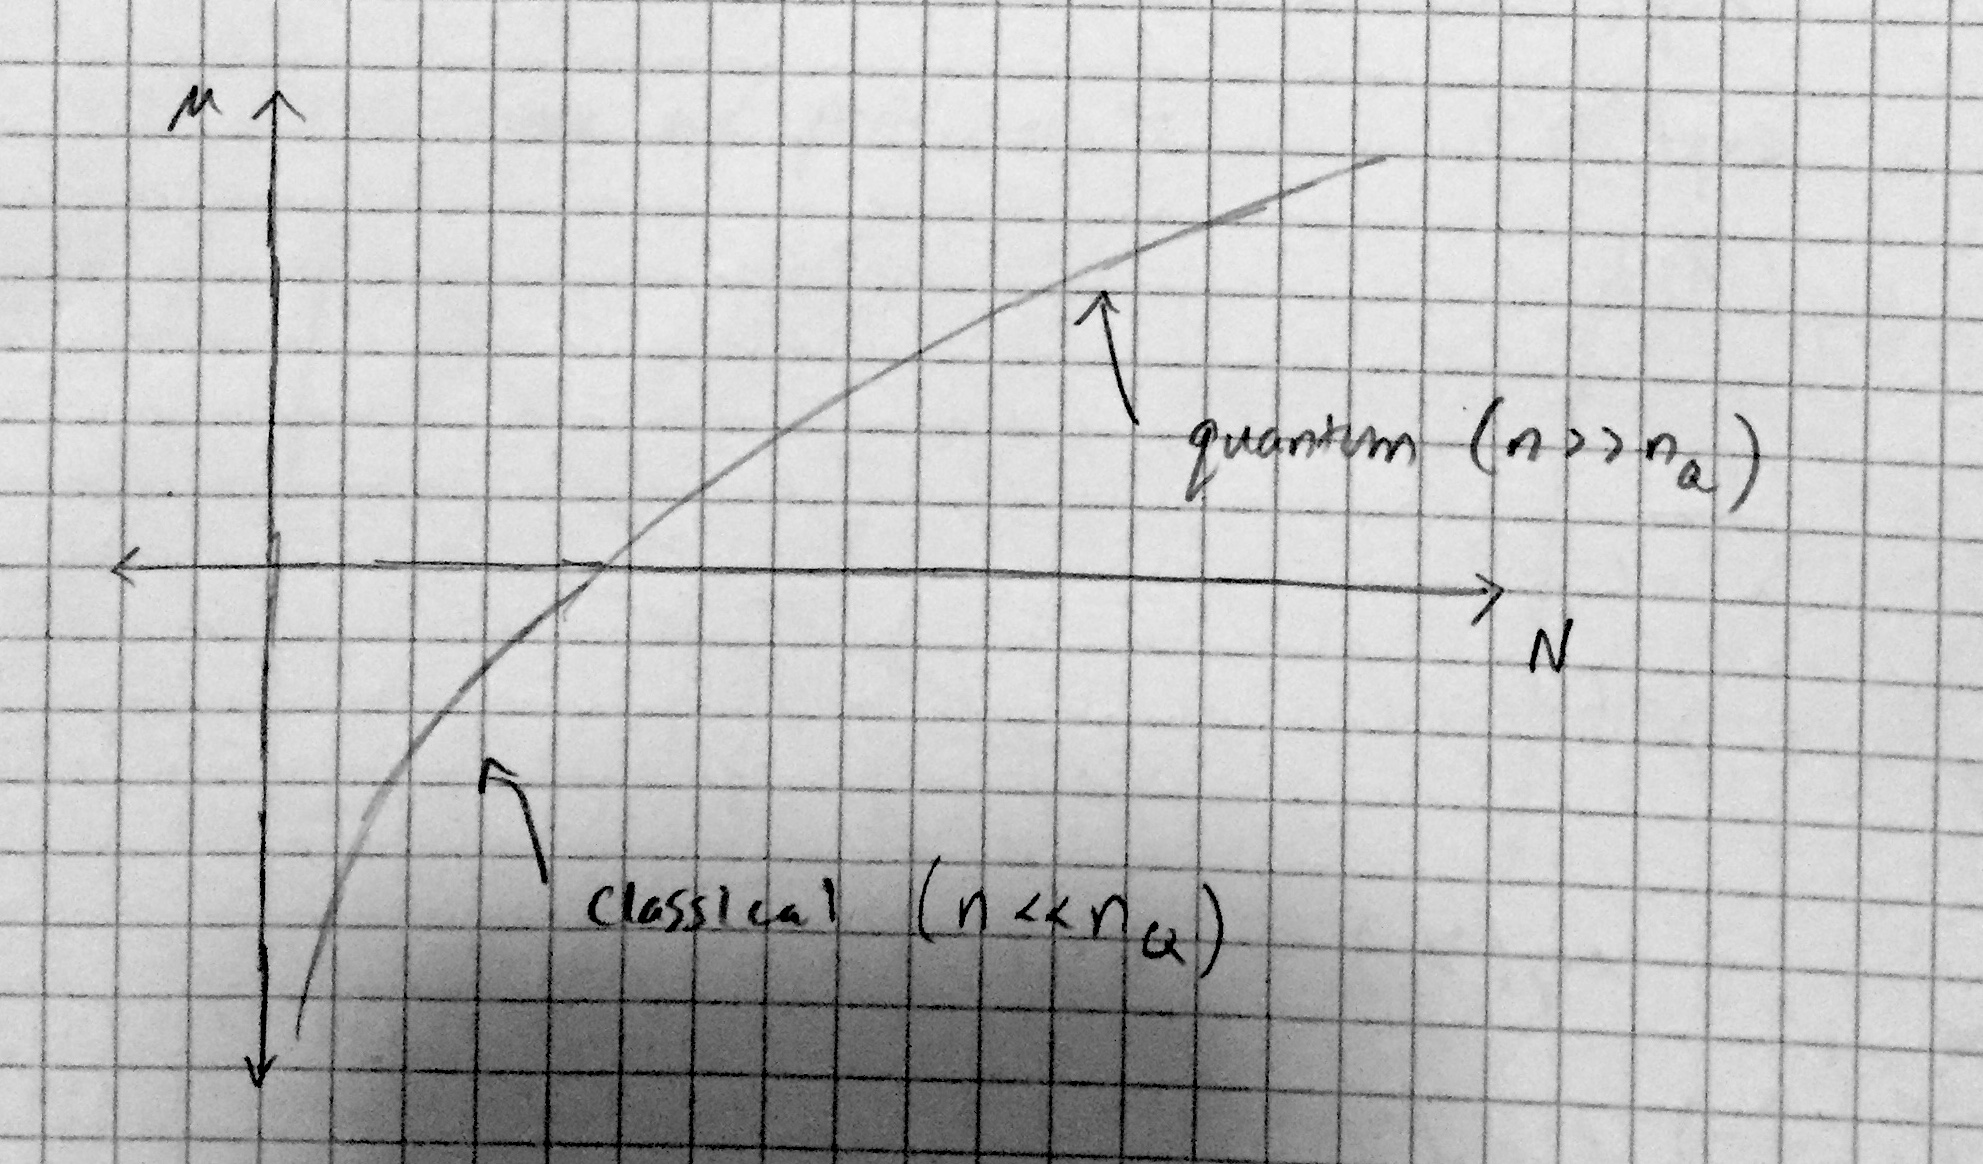
\includegraphics[width=12cm]{img/fermi}
	\end{figure}

	\item

	If there are $N_0$ atoms in the ground state and $N_1$ particles in the first excited state, $N_0 = 2N_1$ and $N_1 + N_2 = N$, then

	$$N_0 = \frac{2}{3}N = (\exp(-\mu/\tau)-1)^{-1}$$

	and

	$$N_1 = \frac{1}{3}N = (\exp(\epsilon-\mu/\tau)-1)^{-1}.$$

	Then, taking $\lambda = \exp(\mu/\tau),$

	\begin{gather*}
	2 = \frac{\lambda^{-1}\exp(\epsilon/\tau) - 1}{\lambda^{-1} -1} \\
	2\lambda^{-1} - 1 = \lambda^{-1}\exp(\epsilon/\tau) \\
	2 - \lambda = \exp(\epsilon/\tau).
	\end{gather*}

	But

	\begin{gather*}
	\frac{2}{3}N = \frac{1}{\lambda^{-1} - 1} \\ 
	\frac{3}{2N} + 1= \lambda^{-1},
	\end{gather*}

	so

	$$2 - \frac{1}{1 + (3/2N)} = \exp(\epsilon/\tau).$$

	But $N \gg 1$, so using the approximation $(1+x)^{-1} \approx 1-x$ for small $x$,

	\begin{gather*}
	2 - \left( 1 - \frac{3}{2N} \right) = \exp(\epsilon/\tau) \\
	1 + \frac{3}{2N} = \exp(\epsilon / \tau) \\
	\log\left(1 + \frac{3}{2N}\right) = \frac{\epsilon}{\tau}.
	\end{gather*}

	Once again, in the limit $N \gg 1$, we can use the approximation $\log (1+x) \approx x$ for small $x$, so

	\begin{gather*}
	\frac{3}{2N} = \frac{\epsilon}{\tau} \\
	\tau = \frac{2N\epsilon}{3}.
	\end{gather*}


	\item

	\begin{enumerate}

		\item

		The energy levels are given by $\epsilon_k = \hbar^2 k^2 / 2m$, and imposing periodic boundary conditions, we see that $k_x =(\pi / L_x) n_x$ (and $k_y$ and $k_z$ are symmetric), so

		$$\epsilon_{n_x, n_y, n_z} = \frac{\hbar^2}{2m} \left( \frac{\pi}{V^{1/3}} \right)^2 (n_x^2 + n_y^2 + n_z^2)$$

		where we have assumed that $L_x = L_y = L_z = V^{1/3}$. Then, the energy of the lowest orbital, where $n_x = n_y = n_z = 1$, is

		$$\epsilon_0 = \frac{3 \hbar^2}{2m} \left( \frac{\pi}{V^{1/3}} \right)^2.$$

		Since we have $V = 10^{-15}$ m$^{3}$ and $m = 87$ u for Rb-87, this gives $\epsilon_0 = 7.11 \times 10^{-14}$ eV.

		\item

		The Einstein temperature is given by

		$$\tau_E = \frac{2 \pi \hbar^2}{m} \left( \frac{N}{2.61V} \right)^{2/3}$$

		which for $N = 10^4$ and $m$ and $V$ as previously, gives $\tau_E = 7.39 \times 10^{-12}$ eV.

		\item

		If $T = 0.9 T_E \implies \tau = 0.9 \tau_E = 6.65 \times 10^{-12}$ eV, then the number of particles in the ground state is 

		$$N_0 = N - N_e(\tau) = N - 2.612 V \left( \frac{m \tau}{2 \pi \hbar^2} \right)^{3/2} = 1.46 \times 10^3.$$

		The chemical potential is $\mu = \epsilon_0 - (\tau / N_0) = 6.66 \times 10^{-14}$ eV, or $4.56 \times 10^{-14}$ eV less than the ground state energy.

		The number of particles in each of the threefold-degenerate first excited states, which have energy

		$$\epsilon_1 = \frac{3\hbar^2}{m} \left( \frac{\pi}{V^{1/3}} \right)^2 = 1.42 \times 10^{-13} \text{ eV}$$

		is

		$$N_1 = \frac{1}{\exp((\epsilon_1 - \mu)/ \tau) -1} = 99.$$

		\item

		For $N = 10^6$, $\tau_E = 1.59 \times 10^{-10}$ eV. So $\tau = 0.9 \tau_E = 1.43 \times 10^{-10}$ eV.

		Thus $N_0 = N - N_e(\tau) = 1.48 \times 10^5$.

		Then $\mu = \epsilon_0 - (\tau / N_0) = 7.11 \times 10^{-14}$, or $9.66 \times 10^{-17}$ less than the ground state energy.

		And the number of particles in each of the first excited states is $2.0 \times 10^3$.

		We see there are relatively more particles in the ground state as the number of particles $N$ increases because the chemical potential is increasingly closer to the ground state energy. So when $\Delta \epsilon \gg \mu \implies \epsilon_1 \gg (\tau / N)$, the number of particles in the ground state is much greater than the number of particles in the first excited state.

	\end{enumerate}

	\item

	\begin{enumerate}

		\item

		For a one-dimensional system, imposing periodic boundary conditions on a line of length $L$ such that $k = \pi n/ L$

		$$\epsilon(n) = \frac{\hbar^2}{2m}k^2 = \frac{\hbar^2}{2m} \frac{\pi^2}{L^2} n^2 \implies n = \frac{2mL^2}{\hbar^2\pi^2} \epsilon^{1/2},$$

		thus

		$$\mathcal{D}(\epsilon) = \frac{d n}{d\epsilon} = \frac{mL^2}{\hbar^2\pi^2} \epsilon^{-1/2}.$$

		So the total number of particles in excited orbitals can be approximated by the integral

		$$N_\epsilon = \int \limits_0^{\infty} f(\epsilon, \tau) \; dn = \int \limits_0^{\infty} \mathcal{D}(\epsilon) f(\epsilon, \tau) \; d\epsilon$$

		where $f(\epsilon, \tau) = (\exp((\epsilon - \mu) / \tau) - 1)^{-1} = (\lambda^{-1} \exp(\epsilon / \tau) - 1)^{-1}$ is the Bose-Einstein occupancy function. Thus

		$$N_\epsilon = \frac{2mL^2}{\hbar^2\pi^2} \int \limits_0^{\infty} \frac{\epsilon^{-1/2}}{\lambda^{-1} \exp(\epsilon / \tau) - 1} d\epsilon.$$

		For $\lambda = 1$, this becomes

		$$N_\epsilon = \frac{2mL^2}{\hbar^2\pi^2} \tau^{1/2} \int \limits_0^{\infty} \frac{x^{-1/2}}{\exp(x) - 1} dx,$$

		which does not converge.

		\item

		For the integral to converge, the density of states must contain a factor of $\epsilon$ with an exponent $\geq 0$. For a $d$-dimensional system, if we impose symmetry in $k$-space,

		$$D(\epsilon) = \frac{d^dn}{d\epsilon} \propto \epsilon^{-1/2} n^{d-1} dn \propto \epsilon^{(d/2) - 1}.$$

		So the condition for convergence is $(d/2) - 1 \geq 0$, or $d \geq 2$. If the system is at least two-dimensional, there will be an abrupt Bose-Einstein transition.

	\end{enumerate}

\end{enumerate}

\end{document}